% ============================================================================
% Anexo C --- Coordinaci\'on de Protecciones
% Proyecto: Generacion Distribuida 990 kW - Puerto Boyaca (EBSA), circuito 15344
% Generado automaticamente por scripts/Anexos.py - no editar a mano.
% Compilador recomendado: pdfLaTeX.
% ============================================================================
\documentclass[11pt,a4paper]{article}

\usepackage[spanish,es-tabla]{babel}
\usepackage[utf8]{inputenc}
\usepackage[T1]{fontenc}
\usepackage{textcomp}

\usepackage[a4paper,margin=2.5cm]{geometry}
\usepackage{fancyhdr}
\usepackage{titlesec}
\usepackage{setspace}
\onehalfspacing

\usepackage{booktabs}
\usepackage{longtable}
\usepackage{array}
\usepackage{tabularx}
\usepackage{graphicx}
\usepackage{caption}
\usepackage{float}
\usepackage{siunitx}
\sisetup{output-decimal-marker={,}, group-separator={.}}

\usepackage{enumitem}
\usepackage[dvipsnames]{xcolor}
\usepackage[colorlinks=true,linkcolor=NavyBlue,citecolor=NavyBlue,urlcolor=NavyBlue]{hyperref}

\graphicspath{{figuras/}{../}}

\pagestyle{fancy}
\fancyhf{}
\fancyhead[L]{Anexo C --- Coordinaci\'on de Protecciones}
\fancyhead[R]{\thepage}
\fancyfoot[C]{\small Confidencial -- Uso exclusivo tr\'amite de conexi\'on ante EBSA}
\renewcommand{\headrulewidth}{0.4pt}

\titleformat{\section}{\normalfont\Large\bfseries}{\thesection.}{0.6em}{}
\titleformat{\subsection}{\normalfont\large\bfseries}{\thesubsection}{0.6em}{}

\begin{document}

\begin{titlepage}
\centering
\vspace*{3cm}
{\Large\bfseries Estudio de Conexi\'on Simplificado\par}
\vspace{0.4cm}
{\large Generaci\'on Distribuida 990\,kW --- Puerto Boyac\'a\par}
\vspace{0.2cm}
{\large Circuito 15344 --- EBSA --- Solicitud N.\textdegree{} 16869\par}
\vspace{2.5cm}
{\Huge\bfseries Anexo C --- Coordinaci\'on de Protecciones\par}
\vspace{2cm}
{\large Resoluci\'on CREG 174 de 2021\par}
\vfill
{\small Documento generado autom\'aticamente a partir de los resultados de simulaci\'on.\par}
\end{titlepage}

\tableofcontents
\newpage


\section{Alcance y metodolog\'ia}

Este anexo recoge el detalle de la comprobaci\'on de coordinaci\'on que sustenta
la Secci\'on 9.2 y el anexo de protecciones del informe principal.

\subsection{Qu\'e se comprueba}

No se trata de diseñar de nuevo la protecci\'on del circuito, sino de verificar
si el \textbf{ajuste ya aprobado y en operaci\'on} del reconectador de cabecera
del circuito 15344 sigue coordinando correctamente una vez se agrega el aporte
de falla del proyecto.

\subsection{F\'ormula aplicada}

Curva IEC Normal Inverse, seg\'un IEC 60255-151 --- la misma familia con la que
el Operador de Red ajust\'o la protecci\'on de cabecera:
\[
t(I) = \mathrm{Dial} \cdot \frac{k}{\left(I/I_{arranque}\right)^{\alpha} - 1},
\qquad k = 0.14,\quad \alpha = 0.02
\]

Si la corriente supera el umbral instant\'aneo, el rel\'e no espera la curva
temporizada y opera en tiempo definido corto.

\subsection{Ajustes evaluados}

\small
\begin{longtable}{lrl}
\toprule
\textbf{Parámetro} & \textbf{Valor} & \textbf{Unidad} \\
\midrule
\endfirsthead
\toprule
\textbf{Parámetro} & \textbf{Valor} & \textbf{Unidad} \\
\midrule
\endhead
\bottomrule
\endfoot
Curva & IEC Normal Inverse & --- \\
Arranque 51 & 240.0 & A \\
Dial 51 & 0.10 & --- \\
Instantáneo 50 & 1500.0 & A \\
Arranque 51N & 60.0 & A \\
Dial 51N & 0.10 & --- \\
Instantáneo 50N & 300.0 & A \\
Tiempo de recierre rápido & 2.0 & s \\
\end{longtable}
\vspace{-0.5em}
{\small\itshape Ajustes reales de la protecci\'on de cabecera, seg\'un el documento de insumos del Operador de Red.}


\newpage\section{Curva tiempo-corriente}

\begin{figure}[H]
\centering
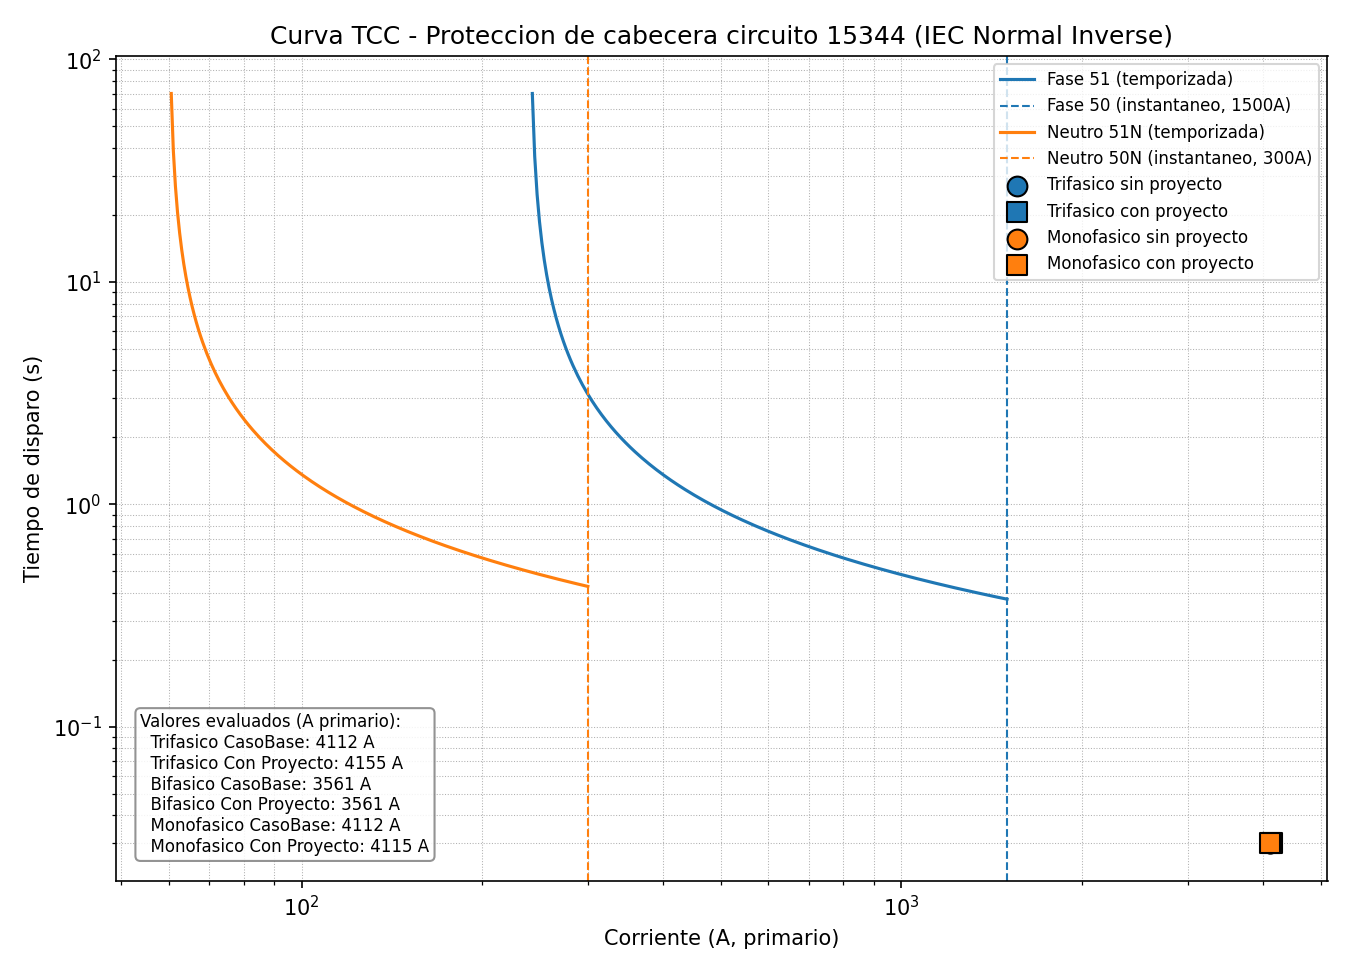
\includegraphics[width=1.0\textwidth]{Curva_TCC_Cabecera_15344.png}
\caption{Curva TCC de la protecci\'on de cabecera, con los puntos de falla evaluados.}
\label{fig:anexoC-tcc}
\end{figure}

\newpage\section{Resultados}

\subsection{Comparativa Cabecera 15344}

\small
\begin{longtable}{lllllllll}
\toprule
\textbf{C1} & \textbf{C2} & \textbf{C3} & \textbf{C4} & \textbf{C5} & \textbf{C6} & \textbf{C7} & \textbf{C8} & \textbf{C9} \\
\midrule
\endfirsthead
\toprule
\textbf{C1} & \textbf{C2} & \textbf{C3} & \textbf{C4} & \textbf{C5} & \textbf{C6} & \textbf{C7} & \textbf{C8} & \textbf{C9} \\
\midrule
\endhead
\bottomrule
\endfoot
Trifasico & 51/50 (fase) & CasoBase & 4.112 & 4112.041 & Instantaneo & 0.030 &  &  \\
Trifasico & 51/50 (fase) & Con\_Proyecto & 4.155 & 4155.350 & Instantaneo & 0.030 & 43.309 & 1.053 \\
Bifasico & 51/50 (fase) & CasoBase & 3.561 & 3561.132 & Instantaneo & 0.030 &  &  \\
Bifasico & 51/50 (fase) & Con\_Proyecto & 3.561 & 3561.133 & Instantaneo & 0.030 & 0.001 & 0.000 \\
Monofasico & 51N/50N (neutro) & CasoBase & 3.770 & 3770.160 & Instantaneo & 0.030 &  &  \\
Monofasico & 51N/50N (neutro) & Con\_Proyecto & 3.774 & 3774.327 & Instantaneo & 0.030 & 4.167 & 0.111 \\
\end{longtable}

\subsection{Aporte Falla Generacion}

\small
\begin{longtable}{llll}
\toprule
\textbf{Parametro} & \textbf{Valor} & \textbf{Unidad} & \textbf{Fuente} \\
\midrule
\endfirsthead
\toprule
\textbf{Parametro} & \textbf{Valor} & \textbf{Unidad} & \textbf{Fuente} \\
\midrule
\endhead
\bottomrule
\endfoot
Ik"3PF configurado por inversor & 238.200 & A & PowerFactory - ElmPvsys, pestana Short-Circuit VDE/IEC \\
Cantidad de inversores & 3 & - & Ficha tecnica Huawei SUN2000-330KTL-H1 \\
Corriente nominal del inversor (calculada) & 238.157 & A & 330kW / (raiz(3) x 800V), cos(phi)=1 \\
Aporte configurado en p.u. de la corriente nominal & 1.000 & p.u. & Calculado \\
Limite regulatorio (Anexo 1, Acuerdo CNO 2121/2026) & 1.100 & p.u. & Anexo\_1\_Acuerdo\_2121.pdf \\
Ikss trifasico validado en barra propia del generador & 0.715 & kA & Resultados\_Cortocircuito.xlsx (corrida real) \\
Nota & Este valor (corriente de falla trifasica real del sistema de generacion, segun la simulacion) es el insumo a usar para el diseno de la malla de puesta a tierra del proyecto. & - & - \\
\end{longtable}

\subsection{Selectividad Proyecto}

\small
\begin{longtable}{llllll}
\toprule
\textbf{C1} & \textbf{C2} & \textbf{C3} & \textbf{C4} & \textbf{C5} & \textbf{C6} \\
\midrule
\endfirsthead
\toprule
\textbf{C1} & \textbf{C2} & \textbf{C3} & \textbf{C4} & \textbf{C5} & \textbf{C6} \\
\midrule
\endhead
\bottomrule
\endfoot
Corriente de falla referida a 13.2 kV [A] & 858.400 &  &  &  &  \\
Proteccion & Arranque [A] & Dial & I/Iarranque & Zona & Tiempo de disparo [s] \\
Proyecto (51, punto de conexion) & 70 & 0.050 & 12.260 & Temporizado & 0.136 \\
Cabecera circuito 15344 (51) & 240 & 0.100 & 3.580 & Temporizado & 0.542 \\
Margen de selectividad [s] & 0.406 & CUMPLE (>= 0.2 s) &  &  &  \\
Verificacion anti-isla frente al recierre de cabecera &  &  &  &  &  \\
Recierre rapido de cabecera [s] & 2 & Dato EBSA (DOC\_REF\_EST pag. 4) &  &  &  \\
Desconexion del proyecto [s] & 1 & Funciones 27/59/81/81R &  &  &  \\
Margen antes del recierre [s] & 1 & CUMPLE (>= 0.5 s) &  &  &  \\
\end{longtable}

\subsection{Conclusion}

\small
\begin{longtable}{l}
\toprule
\textbf{Detalle por tipo de falla} \\
\midrule
\endfirsthead
\toprule
\textbf{Detalle por tipo de falla} \\
\midrule
\endhead
\bottomrule
\endfoot
- Falla trifasico en cabecera 15344: 4112A -> 4155A (+1.05\%), ambos en zona 'Instantaneo' con el mismo tiempo de disparo (0.030s) -> NO requiere reajuste. \\
- Falla bifasico en cabecera 15344: 3561A -> 3561A (+0.00\%), ambos en zona 'Instantaneo' con el mismo tiempo de disparo (0.030s) -> NO requiere reajuste. \\
- Falla monofasico en cabecera 15344: 3770A -> 3774A (+0.11\%), ambos en zona 'Instantaneo' con el mismo tiempo de disparo (0.030s) -> NO requiere reajuste. \\
Conclusion general \\
No se requiere reajuste de la proteccion de cabecera del circuito 15344: el aporte de falla del proyecto es marginal frente al nivel de cortocircuito de la red de EBSA y ambos escenarios (sin y con proyecto) siguen operando en la misma zona de la curva ya aprobada. \\
\end{longtable}

\end{document}